% TODO überarbeiten, da Beispielproblem rausgezogen wurde
%      - Erklärung für Beispielproblem kürzen
%      - etwas in Thing einbauen, das sich zu vererben lohnt (Diamantproblem)
%      - Redefinition von Methoden

\section{CLOS}
Grundlage für dieses Kapitel ist das Buch ``Object-Oriented Programming in Common Lisp. A Programmer's Guide to CLOS''\cite{keene} von Sonya E. Keene. 

Das Common Lisp Object System ist der Standard für objektorientierte Programmierung in der Sprache Common Lisp. Auch Racket bietet es an, in diesem Stil objektorientiert zu programmieren. Um anstatt des Racket-Objektsystems mit CLOS-Objekten zu arbeiten, muss lediglich die Sprache auf den Dialekt Swindle umgestellt werden:


\begin{lstlisting}
#lang swindle
\end{lstlisting}

Wir wollen nun versuchen, die Klassen Thing, Element, Animal und Pokemon auch in CLOS zu schreiben, um zu sehen, welche Unterschiede in der Syntax es gibt und wie Mehrfachvererbung hier umgesetzt ist. 

Alle Code-Beispiele sind auch noch einmal zusammenhängend in Anhang \ref{clos-example} aufgeführt.

\subsection{Einfache Klassen}
Für die Definition von Klassen in CLOS gibt es das Makro \texttt{defclass}. Im Gegensatz zu dem Objektsystem von Racket erstellt das Makro eine benannte Klasse. Der Name wird beim Aufruf mit übergeben, damit erübrigt sich eine anschließende Benennung mit \texttt{define}. Auch in CLOS wird die Superklasse mit angegeben. Da es jedoch mehrere Superklassen geben kann, werden diese in einer Liste übergeben. Hat die Klasse keine Superklassen (außer der Wurzelklasse), so wird die leere Liste übergeben. Die explizite Angabe der Wurzelklasse als Superklasse nicht nicht nötig. Anschließend können noch die Slots der Klasse angegeben werden. Für eine minimale Klasse ohne Superklasse(n) genügt der Name und die leere Liste: 

\begin{lstlisting}
((defclass Thing ())
\end{lstlisting}

% Zur Objekterzeugung gibt es in CLOS zwei verschiedene Möglichkeiten, je nachdem ob \texttt{:automaker} als Klassen-Option gesetzt wurde oder nicht. 

Objekte dieser Klasse können mit dem Schlüsselwort \texttt{make} erzeugt werden.

\begin{lstlisting}
> (make Thing)
\end{lstlisting}
{\routput \#Thing}

Felder (oder Slots, wie sie in CLOS üblicherweise genannt werden) werden nach der Superklasse angegeben. Ein großer Unterschied zu dem Objektsystem von Racket ist, dass innerhalb einer Klassendefinition \textit{nur} Slots definiert werden, keine Methoden. Methoden werden außerhalb der Klasse definiert. Das bedeutet, dass kein Schlüsselwort benötigt wird, um anzugeben, ob gerade ein Slot oder eine Methode definiert wird. Wir können also für die Definition der Klasse Element beispielweise einfach schreiben:

\begin{lstlisting}
(defclass Element (Thing)
  attr)
\end{lstlisting}

Die Klasse hat genau einen Slot namens \texttt{attr}, der jedoch so noch nicht sehr nützlich ist.

Damit mit diesem Slot auch interargiert werden kann, benötigt er noch Accessoren: einen Getter (in CLOS Reader genannt) und einen Setter (in CLOS Writer genannt). Außerdem möchte man gegebenenfalls einen Initialwert angeben können, den Slot dokumentieren, typisieren und so weiter. All dies geschieht durch Slot-Optionen. Sie folgen nach dem Namen des Slots (der nun geklammert werden muss, damit klar ist, wann die Slot-Definition zuende ist) und beginnen per Konvention mit einem Doppelpunkt. Um auf das Attribut \texttt{attr} beispielsweise lesend oder schreibend zugreifen zu können, kann die Slot-Option \texttt{:reader} beziehungsweise \texttt{:writer} gesetzt werden oder, falls beides über das gleiche Schlüsselwort möglich sein soll, auch die Option \texttt{:accessor}. Accessoren müssen benannt werden. Im Gegensatz zu dem Objektsystem von Racket muss sich der Name jedoch nicht vom Namen des Slots unterscheiden. Hier also die vollständige Definition der Klasse:

\begin{lstlisting}
(defclass Element (Thing)
  (attr
    :accessor attr
    :initvalue 'water
    :initarg :attr)
  :printer #t
  :automaker #t)
\end{lstlisting}

Für die Klasse gibt es drei nützliche Slot- und Klassenoption: \texttt{:initarg}, \texttt{:printer} und \texttt{:automaker}. Die \texttt{:initarg}-Option bewirkt, dass der Parameter bei der Objekterzeugung initialisiert werden kann.

\begin{lstlisting}
(make Element :attr 'fire)
\end{lstlisting}

Durch die \texttt{:printer}-Option erhalten wir bei Aufruf der \texttt{print}-Funktion an einem Objekt oder bei Auswertung des Objekts in der Direkteingabe einen formattierten String. Das hat den Vorteil, dass zur Überprüfung des Zustandes des Objekts nicht jeder Slot einzeln abgefragt werden muss.

\begin{lstlisting}
> (make Element)
\end{lstlisting}
{\routput \#<Element: attr=water>}

\texttt{:automaker} bewirkt, dass es zusätzlich zu dem Schlüsselwort \texttt{make} zur Erzeugung von allgemeinen Objekten nun auch das Schlüsselwort \texttt{make-Element} zur Erzeugung von Objekten der Klasse Element gibt. Element-Objekte können natürlich auch weiterhin mit \texttt{make} erzeugt werden.

\begin{lstlisting}
(make Element :attr 'fire)
(make-Element 'fire)
\end{lstlisting}

Der Wert eines Slots, der einen Writer oder Accessor besitzt, kann nach der Objekterzeugung mittels \texttt{set!} verändert werden:

\begin{lstlisting}
(define elem (make Element))
> (set! (attr elem) 'wind)
> (attr elem)
\end{lstlisting}
{\routput wind}

Eine weitere nützliche Klassenoption ist \texttt{:autoaccessors :slot}, die automatisch für jeden Slot Accessor-Funktionen generiert. Der Name der Accessor-Funktion ist dann identisch zum Slot. Wir verwenden sie für die Klasse Animal.

\begin{lstlisting}
(defclass Animal (Thing)
  (gender :initvalue 'male)
  (size   :initvalue 'small)
  :autoaccessors :slot
  :automaker #t
  :printer #t)
\end{lstlisting}

Da im folgenden die Objekte nur noch mit \texttt{make-Animal} erzeugt werden, wurde die \texttt{:initarg}-Option weggelassen. Es können beliebig viele Argumente an \texttt{make-Animal} übergeben werden, im Zweifelsfalls werden die Slots mit Standardwerten belegt oder überschüssige Parameter ignoriert.

\begin{lstlisting}
> (make-Animal)
\end{lstlisting}
{\routput \#<Animal: gender=male size=small>}

\begin{lstlisting}
> (make-Animal 'female)
\end{lstlisting}
{\routput \#<Animal: gender=female size=small>}

\begin{lstlisting}
> (make-Animal 'female 'normal 42)
\end{lstlisting}
{\routput \#<Animal: gender=female size=normal>}

\subsection{Mehrfachvererbung in CLOS}
Für Mehrfachvererbung in CLOS genügt es, mehr als eine Klasse in der Liste der Superklassen anzugeben. Um eine Klasse Pokemon aus Element und Animal zu definieren können wir also schreiben:

\begin{lstlisting}
(defclass Pokemon (Animal Element)
    :automaker #t
    :printer #t)
\end{lstlisting}

Objekte der Klasse erben automatisch alle Slots.

\begin{lstlisting}
> (make-Pokemon)
\end{lstlisting}
{\routput \#<Pokemon: attr=water gender=male size=small>}

\begin{lstlisting}
> (make-Pokemon 'fire 'female 'large)
\end{lstlisting}
{\routput \#<Pokemon: attr=fire gender=female size=large>}

Die Klasse kann auch noch weitere Slots definieren. Wollen wir, dass jedes Pokemon sich seinen Index im Pokedex merkt, so wird sie um den neuen Slot ergänzt.

\begin{lstlisting}
 (defclass Pokemon (Animal Element)
  (index :initvalue 0)
  :autoaccessors :slot
  :automaker #t
  :printer #t)
\end{lstlisting}

Objekte der Klasse haben nun vier Slots.

\begin{lstlisting}
(define p1 (make-Pokemon))
(define p2 (make-Pokemon 'fire 'female 'large 42))
> p1
\end{lstlisting}
{\routput \#<Pokemon: attr=water gender=male size=small index=0>}

\begin{lstlisting}
> p2
\end{lstlisting}
{\routput \#<Pokemon: attr=fire gender=female size=large index=42>}

Die Liste von Superklassen in einer Klassendefnition wird auch Klassenpräzendenzliste genannt. Sie bestimmt im Zweifel von Konflikten, welche Slots oder Methoden (im Standardfall) vererbt werden. Die am weitesten links stehende Klasse ist die spezifischste, die am weitesten rechts stehende die unspezifischste. Bei Slots kann die Vererbung nicht beeinflusst werden, es wird immer der Slot des am weitesten links in der Liste stehenden Klasse (die diesen Slot bereitstellt) genommen. Auf die Klassenpräzedenz wird noch im Detail im Kapitel \ref{cpl} eingegangen.

Angenommen, es gibt sowohl in Element als auch Animal einen Slot für die Farbe. Dann erbt die Klasse Pokemon immer die Farbe der Klasse Animal, da diese am weitesten links in der Liste steht.

\begin{lstlisting}
(defclass Element ...
  (color :initvalue 'blue))
  
(defclass Animal ...
  (color :initvalue 'brown))

> (make-Pokemon)
\end{lstlisting}
{\routput \#<Pokemon: attr=water color=brown gender=male size=small index=0>}

Nachdem wir gesehen haben, wie Slots vererbt werden, wollen wir uns nun Methoden anschauen.

\subsection{Generische Funktionen und Methodenkombination}
Methoden werden in Racket mit \texttt{defmethod} definiert. Wie bereits erwähnt, werden Methoden in CLOS nicht innerhalb der Klassendefinition definiert, sondern außerhalb. Das Objekt, auf das die Methode angewendet werden soll, wird als Parameter übergeben. Der Typ des Parameters bestimmt demnach, welcher Klasse eine Methode zugeordnet ist. Es ist möglich, eine Methode auf mehrere Klassen zu spezialisieren. Die Objekt-Paramater kommen, falls die Methode zusätzliche Parameter hat, per Konvention an erster Stelle, es ist jedoch prinzipiell jede Reihenfolge möglich. Gibt es keinen Objekt-Parameter, verhält sich das Makro genauso wie \texttt{define}.

Die Methode \texttt{attack}, die für Animal die Größe und für Element das Attribut zurückgibt, kann wie folgt definiert werden.

\begin{lstlisting}
(defmethod attack ((e Element))
  (attr e))

(defmethod attack ((a Animal))
  (size a))
\end{lstlisting}

An die Klasse Pokemon wird, falls wir nichts weiter festlegen, analog zu den Slots die spezifischste Methode vererbt, also die von Animal. Stattdessen sollen beide Werte in einer Liste zu vereint werden. Eine Methode, die auf Pokemon spezialisiert ist, würde das Problem lösen, aber CLOS bietet für die Kombination der Methoden aller (Ober-)Klassen einen Automatismus: generische Funktionen und Methodenkombination. 

Die generische Funktion beschreibt, wie sich das Ergebnis aus den Ergebnissen der Klasse und aller Oberklassen zusammensetzt. Generische Funktionen werden in CLOS mit \texttt{defgeneric} definiert. Tatsächlich gibt es zu jeder Methode, die wir definieren, automatisch eine entsprechende genererische Funktion, selbst wenn wir sie nicht explizit hinschreiben. 

Racket bietet bereits eine Reihe von vordefinierten Methodenkombinationen, wie zum Beispiel für Addition, den logischen Und-Operator, das Maximum oder das Erstellen einer Liste. Falls es für ein Problem keine Standardlösung gibt, können auch eigene Methodenkombinationen definiert werden. Wir benutzen die Listenkombination.

\begin{lstlisting}
(defgeneric attack ((t Thing))
  :combination generic-list-combination)
\end{lstlisting}

Alle von Thing erbenden Klassen geben beim Aufruf von \texttt{attack} nun eine Liste zurück, die alle in der Klassenhierarchie definierten Rückgabewerte der Methoden enthält.

\begin{lstlisting}
> (attack (make Element))
\end{lstlisting}
{\routput (water)}

\begin{lstlisting}
> (attack p2)
\end{lstlisting}
{\routput (big fire)}

Nicht für alle in der Klassenhierarchie vorhanden Klassen muss tatsächlich eine implementierende Methode definiert sein. Die Kombination ist erfolgreich, sobald mindestens eine primäre Methode gefunden wird.

\subsection{Ergänzungsmethoden}
\label{ergmeth}
Für jede der drei Klassen gibt es nun eine \texttt{attack}-Methode, entweder durch Definition mit  \texttt{defmethod} oder aus der generischen Methode mit Methoden-Kombination. Diese Methoden werden Primärmethoden (primary methods) genannt.

Methodenkombination wurde als Methode eingeführt, um geschickt Methoden aus mehreren Superklassen zu verbinden. Tatsächlich geschieht jedoch immer eine Methodenkombination, selbst dann, oder gerade dann wenn, wir sie nicht angeben: die Standard Method Combination.

Sie sorgt zum Beispiel dafür, dass bei einem Methodenaufruf die Primärmethode aufgerufen wird. Aber zusätzlich erlaubt sie es auch, drei spezielle Methoden zu definieren: Vor,- Nach- und Around-Methoden (before, after, around methods). Sie werden zusammenfassend als Ergänzungsmethoden  bezeichnet. Wie der Name vermuten lässt, sind das Methoden, die vor, nach oder um eine Primärmethode herum ausgeführt werden. Sie werden in CLOS mit dem Schlüsselwort \texttt{:before}, \texttt{:after} beziehungsweise \texttt{:around} nach dem Methodennamen definiert.

Nehmen wir beispielsweise eine Klasse für Pokemontrainer. Der tägliche Job eines Trainers ist es, Pokemon zu fangen. Falls er vorher das Haus verlässt und abends zurückkehrt, so lässt sich das in einer Vor- und Nachmethode festhalten:

\begin{lstlisting}
(defclass Trainer ())

(defmethod daily-routine ((t Trainer))
  (display "He caught some Pokemon.\n"))
(defmethod daily-routine :before ((t Trainer))
  (display "He walked out.\n"))
(defmethod daily-routine :after ((t Trainer))
  (display "He walked back home.\n"))
\end{lstlisting}

Weiterhin soll es unter den Pokemontrainern Frühaufsteher geben. Wir halten das Verhalten ebenfalls in drei Methoden fest.

\begin{lstlisting}
(defclass Earlybird (Trainer))

(defmethod daily-routine ((e Earlybird))
  (display "He found two bird Pokemon in the morning.\n"))
(defmethod daily-routine :before ((e Earlybird))
  (display "The sun just started rising.\n"))
(defmethod daily-routine :after ((e Earlybird))
  (display "There was still time before dinner.\n"))
\end{lstlisting}

Im Unterschied zu einer simplen Redefinition oder Erweiterung einer Methode, wird bei Vor- und Nachmethoden sichergestellt, dass keine andere Vor- oder Nachmethode und auch nicht die Primärmethode die Ausführung verhindern kann.

Es werden alle Vormethoden der zwei Klassen, alle Nachmethoden der zwei Klassen sowie der Rumpf der spezifischsten Primärmethode ausgeführt und zwar in folgender Reihenfolge (vgl. \cite[S. 50]{keene}):
\begin{itemize}
 \item Alle Vormethoden, beginnend mit der spezifischsten. Das gibt einer spezifischeren Klasse die Möglichkeit eine Operation auszuführen, die vor allem anderen passiert, inklusive geerbten Vormethoden, der Primärmethode und Nachmethoden.
 \item Die spezifischste Primärmethode. Das erlaubt einer spezifischeren Klasse, die geerbte Methode zu redefinieren.
 \item Alle Nachmethoden, beginnend mit der am wenigstens spezifischen. Das gibt einer spezifischeren Klasse die Möglichkeit eine Operation auszuführen nachdem alles andere passiert ist, inklusive Vormethoden, der Primärmethode und geerbten Nachmethoden.
\end{itemize}

Eine spezifischere Methode hat somit die Möglichkeit, etwas vor beziehungsweise nach dem geerbten Verhalten zu tun. In dem Beispiel mit den Pokemontrainern bedeutet das, dass sich bei einen Aufruf der \texttt{daily-routine}-Methode mit einem Objekt der Klasse Earlybird die folgende Reihenfolge an Methodenaufrufen ergibt:

\begin{figure}[h]
 \centering
 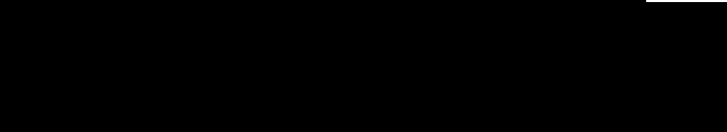
\includegraphics[width=0.9\textwidth]{pictures/primary}
\end{figure}

Natürlich kann jede der Vor- und Nachmethoden vorhanden sein oder nicht. Das einzige, was immer vorhanden sein muss, ist eine anwendbare Primärmethode. Außerdem haben Vor- und Nachmethoden weder Wissen von noch Einfluss auf das Ergebnis der Primärmethode. Sie eignen sich daher nur für Seiteneffekte. Dafür bieten sie der Klasse, die später erweitert wird, eine Möglichkeit, sicherzustellen, dass eine bestimmte Operation garantiert in allen Subklassen ausgeführt wird. Das kann zum Beispiel bei einer Methode zum Malen eines Bildes das Erstellen der Leinwand sein.

Zusätzlich zu Vor- und Nachmethoden gibt es noch Around-Methoden. Sie sind ähnlich zu einer Redefinition mit Super-Aufruf. Die Methode bestimmt selbst, ob und an welcher Stelle in ihrem Rumpf mit \texttt{call-next-method} (das CLOS-Äquivalent zu super) die nächste Methode aufegrufen werden soll. Die Aufrufreihenfolge ist wie folgt (vgl. \cite[S.103]{keene}):
\begin{itemize}
 \item CLOS ruft die spezifischste Around-Methode auf. Sie erhält die gleichen Parameter wie die generische Funktion bzw. Primärmethode.
 \item Falls eine Around-Methode \texttt{call-next-method} aufruft:
 \begin{itemize}
  \item Wenn es weitere anwendbare Around-Methoden gibt, wird die nächstspezifischste aufgerufen und das Ergebnis zurückgegeben.
  \item Ansonsten wird das komplette Framework aus Vor-, Primär- und Nachmethoden aufgerufen und das Ergebnis zurückgegeben.
 \end{itemize}
\end{itemize}

Ein Beispiel für eine Around-Methode ist das Messen der Zeit, die die Primärmethode benötigt. Da Around-Methoden eintscheiden können, \texttt{call-next-method} nicht aufzurufen, können sie den Aufruf aller Vor-, Nach- und Primärmethoden verhindern. Eine Around-Methode muss auch nicht das Ergebnis der Primärmethode zurückgeben (auch wenn es Konvention ist, das zu tun).

Wir haben damit gesehen, dass ein Umgang mit Mehrfachvererbung in CLOS sehr intuitiv und einfach bereitgestellt werden kann.